\documentclass{beamer}

\title{June 11th, 2010 - Boolean Networks}
\author{Bonny Guang, Madison Brandon, Rustin McNeill}
\date{June 11th, 2010}

\begin{document}

\maketitle

%\begin{frame}
% \frametitle{Boolean Models in Biology}
%Why use models in Biology? \\
%\begin{itemize}
%	\item{making and testing a hypothesis}
%\end{itemize}
%Why use a discrete model? \\
%\begin{itemize}
%	\item{easier/cheaper to obtain qualitative information}
%	\item{e.g. gene regulatory networks}
%	\item{still useful for identifying key dynamical features}
%	\item{simple to understand}
%\end{itemize}
%Formula for polynomial form of coordinate functions:
%\[ g_i(x) = \sum_{(c_{i_1}, \ldots, c_{i_r}) \in \mathbb{F}^r} g_i(c_{i_1}, \ldots, c_{i_r}) \prod_{v_j \in I(i)} (` - %(x_j - c_j)^{p - 1}) \]
%When logical model is Boolean, formula simplifies to:
%\[ g_i(x) = \sum_{J \subset I(i)} K_i(J) \prod_{v_j \in J} x_j \prod_{v_j \in I(i)/J} (1 - x_j) \]

%\end{frame}

%\begin{frame}
% \frametitle{Cell Cycle}
%\begin{figure}
%	\centering
%\includegraphics[height=1.8in,width=2.3in,]{cellcycle.png}
%\end{figure}
%Ex: Drosophila cell cycle with proteins $x_1$, $x_2$, $x_3$, $x_4$. \\
%Polynomial functions are: $g_1(x) = 1 + x_2$, $g_2(x) = x_1$, $g_3(x) = 1 + x_1$, $g_4(x) = x_1$. \\
%\end{frame}
%
%\begin{frame}
%\frametitle{State Space for Drosophila example}
%\begin{figure}
%	\centering
%\includegraphics[width=4in]{state_space.jpg}
%\end{figure}
%Determine fixed points and limit cycles in order to understand the dynamics of the cell cycle
%Set each equation equal to its coordinate and solve to get fixed points:
%\[ x_1 = 1 + x_2, x_2 = x_1, x_3 = 1 + x_1, x_4 = x_1 \]
%This system has no fixed points, as we get $x_2 = x_2 + 1$ when we solve.
%\end{frame}

\begin{comment}
%1) 5-state example
%	-more about limit cycles, steady states, components
%	-biological correspondance
%	-in-depth 3-limit cycle
\begin{frame}
 \frametitle{Example with 5 States}
\begin{figure}
    \centering
    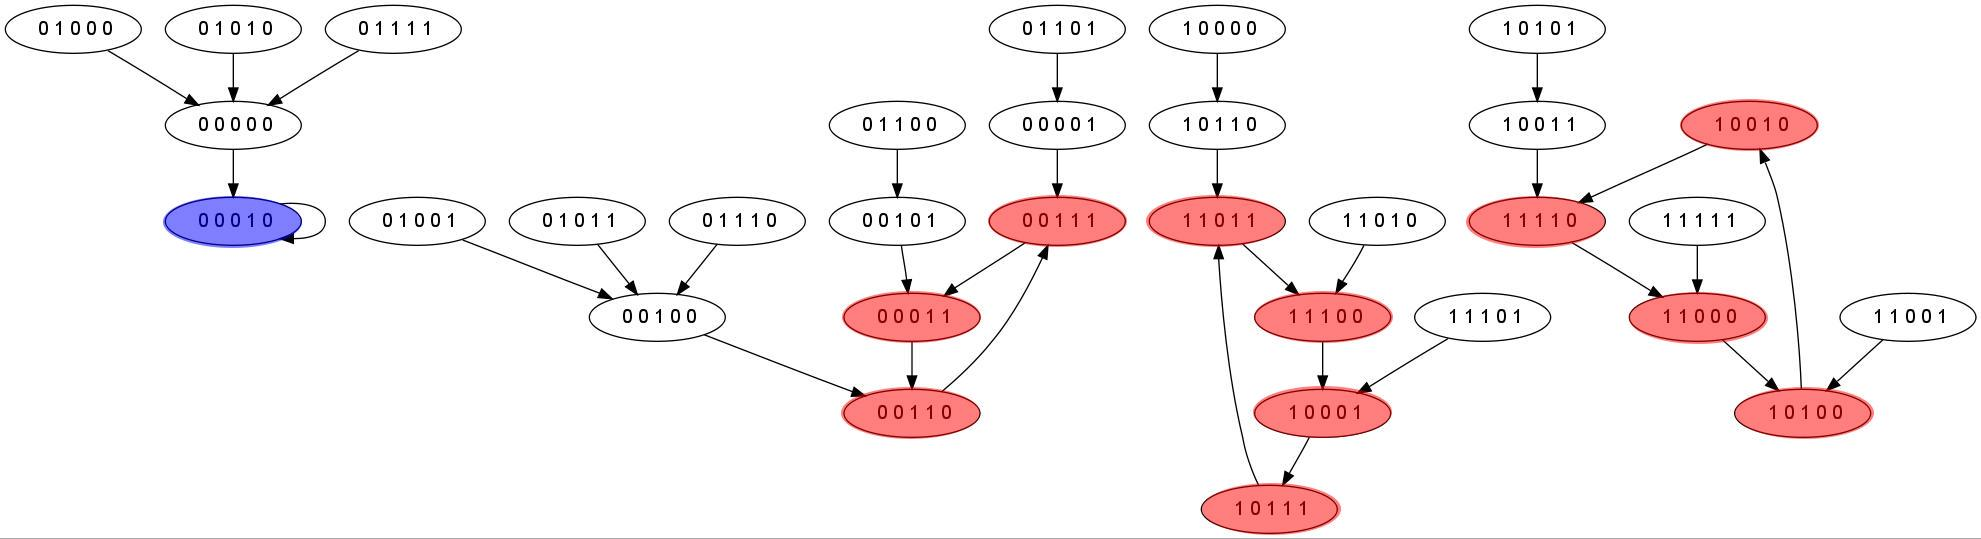
\includegraphics[width = 4in]{5states-1.jpg}
\end{figure}
\begin{itemize}
    \item Can see: 1 fixed point, 1 3-limit cycle, 2 4-limit cycles - total of 4 components \\
    \item Fixed point: point that is mapped to itself by a function \\
    \item Limit cycle: set of points such that all other points in the component approach the cycle \\
\end{itemize}
%Equations that generated this were: $f1 = x1;$ $f2 = x1*x4;$ $f3 = x1 + x5*(1 + x1) + x3;$ $f4 = 1 + x2;$ $f5 = x2*x3 + x3*x4 + (1+x4)*(1+x2)*x5$.
\end{frame}

\begin{frame}
 \frametitle{Closer Look at 3-Limit Cycle}
\begin{figure}
    \centering
    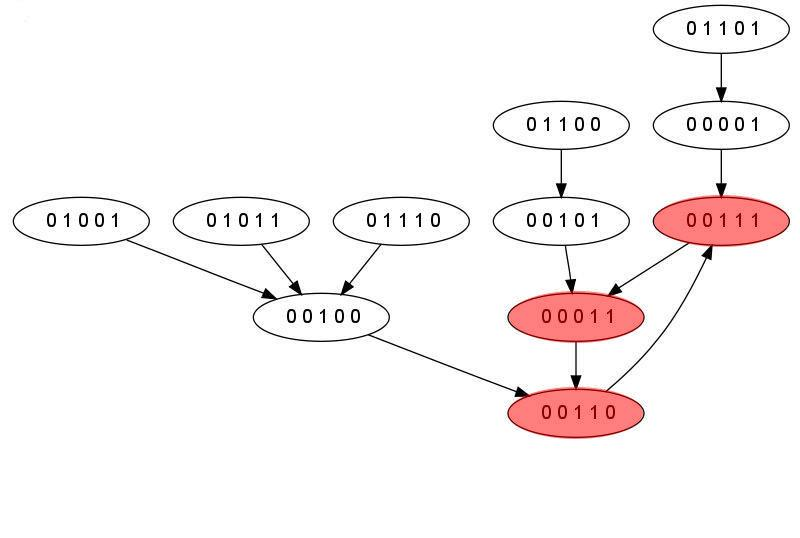
\includegraphics[width = 0.5\textwidth]{limitcycle-1.jpg}
\end{figure}
\begin{itemize}
\item Usually want large components with short cycles
\item Biological meaning: small perturbations in the system won't make it go off somewhere else
\end{itemize}
\end{frame}\end{comment}

\begin{comment}
%2) Limitations of DVD
%	-1000 states
%	-graph of 9 nodes
\begin{frame}
 \frametitle{What Happens As n Gets Bigger?}
\begin{itemize}
 \item DVD can take a max of 1000 nodes.
 \item Let n = 9. Have to graph $2^9 = 512$ nodes.
\end{itemize}
\begin{figure}
    \caption{9 functions plugged into DVD. There are 9 nodes and 2 states.}
    \centering
    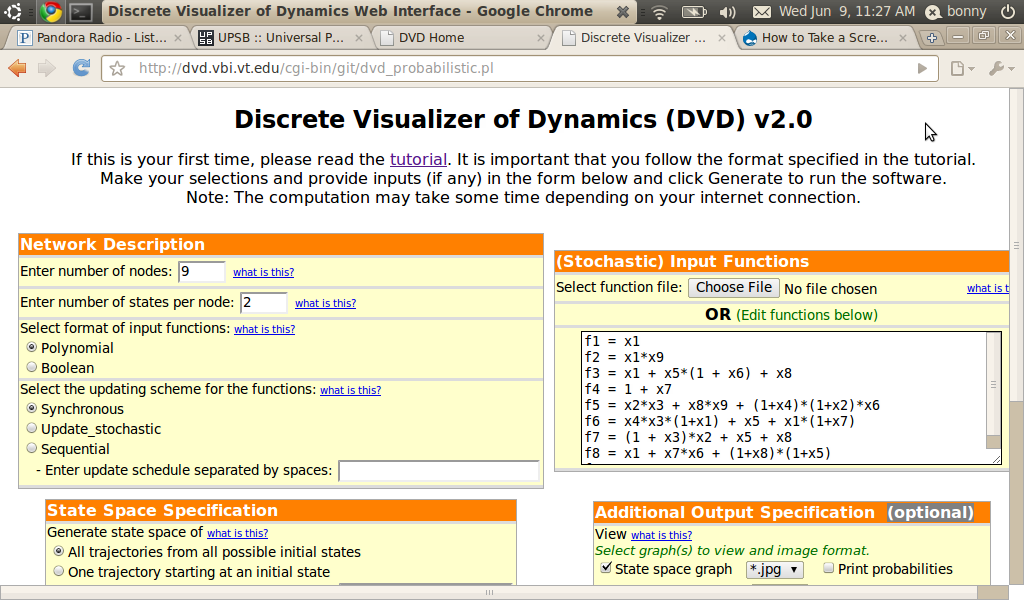
\includegraphics[width = 4in]{dvd1.png}
\end{figure}
\end{frame}

\begin{frame}
\begin{figure}
    \caption{DVD's analysis says that there are 9 components, 4 fixed points of sizes from 2 nodes to 32 nodes.}
    \centering
    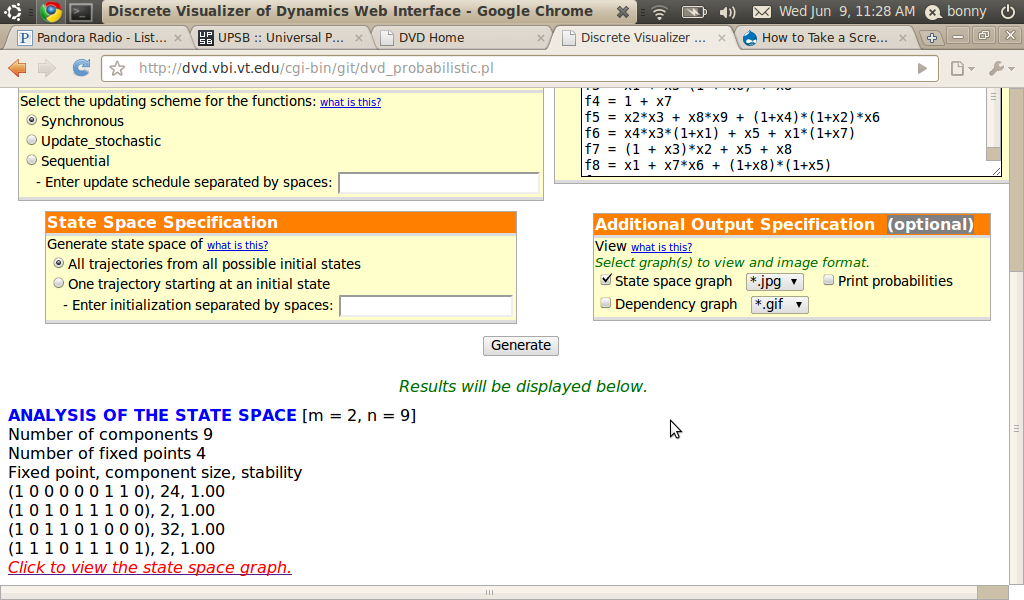
\includegraphics[width = 4in]{dvd2.png}
\end{figure}
\end{frame}
\end{comment}

\begin{frame}
 \frametitle{A Real-Life Wiring Diagram}
\begin{figure}
    \vspace{-10pt}
    \caption{Mammalian cell cycle with at least 60 nodes.}
    \centering
    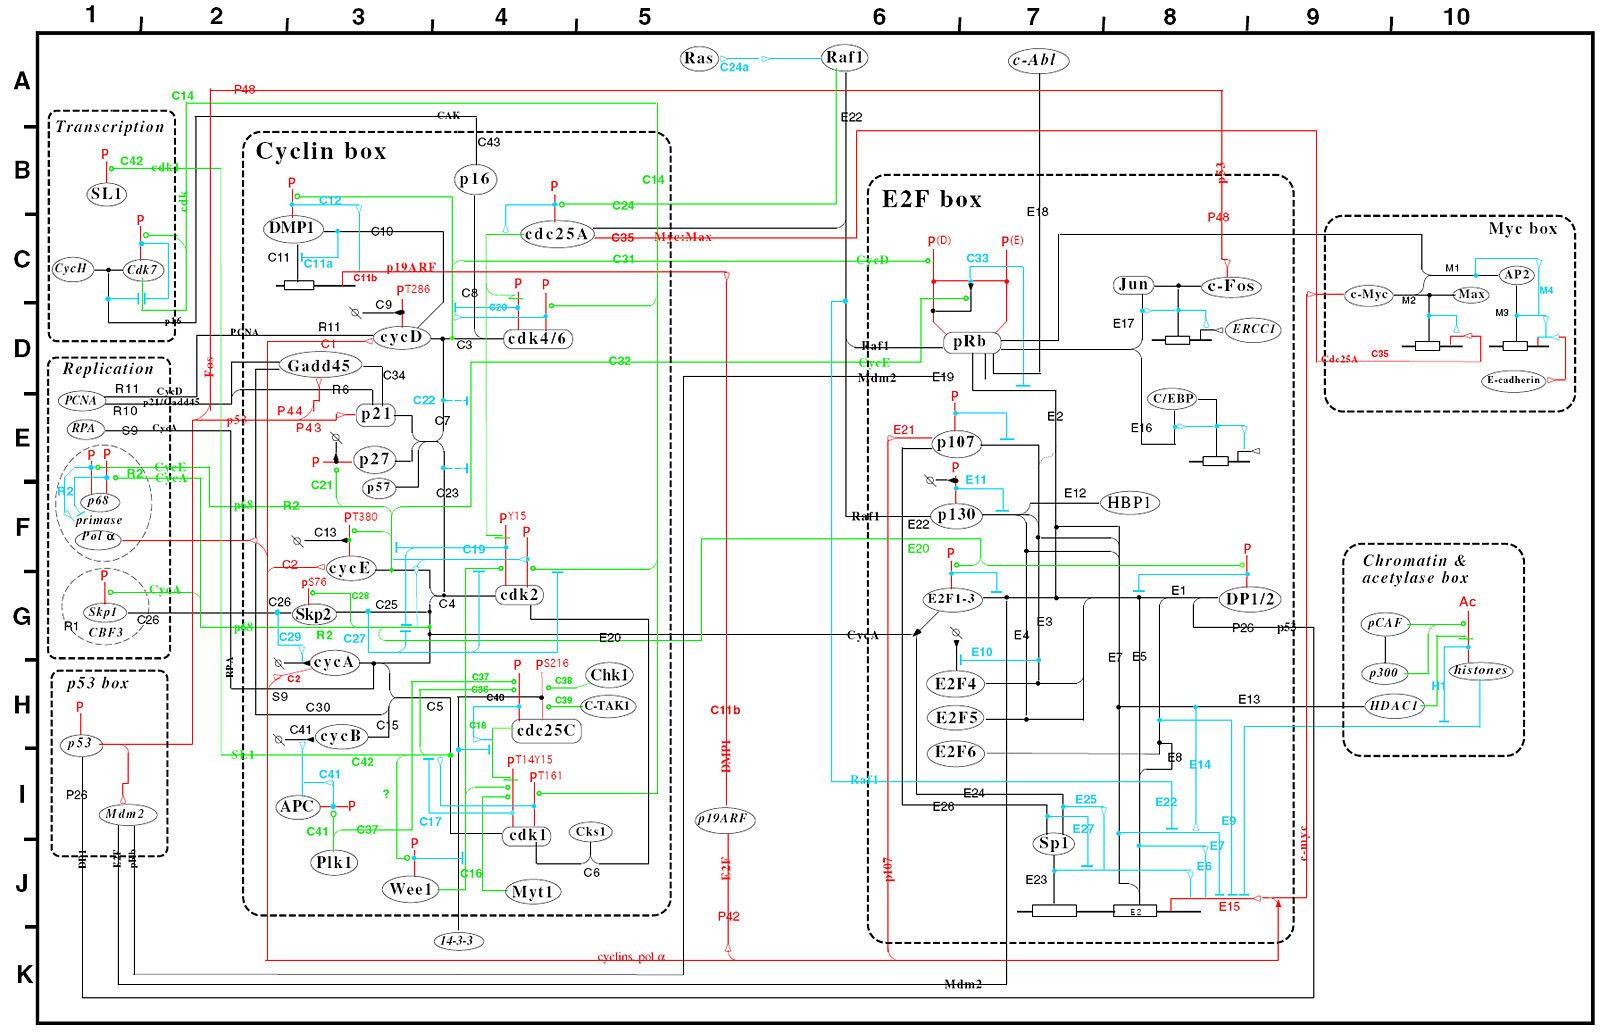
\includegraphics[width = 0.95\textwidth]{hugewiringdiagram.jpg}
    \vspace{-10pt}
\end{figure}
\end{frame}

\begin{frame}
 \frametitle{State Space Diagrams}
\begin{itemize}
 \item $2^{60} \approx 1.2 \times 10^{18}$ states. Let's scale down to $n = 9$ nodes. (DVD online can only take $1000$ states)
 \item Even for $n = 9$, when we try to see the state space graph...
\end{itemize}
\begin{figure}
    \caption{Boolean state space graph, 9 nodes.}
    \centering
    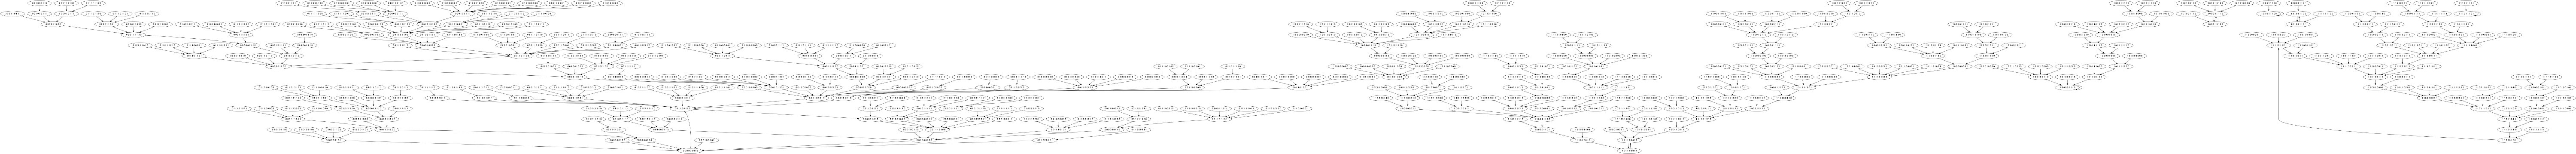
\includegraphics[width = 4in]{9states-1.jpg}
\end{figure}
Impossible to even see the 9 states on one screen!
\begin{figure}
    \caption{Cropping of 3\% of graph}
    \centering
    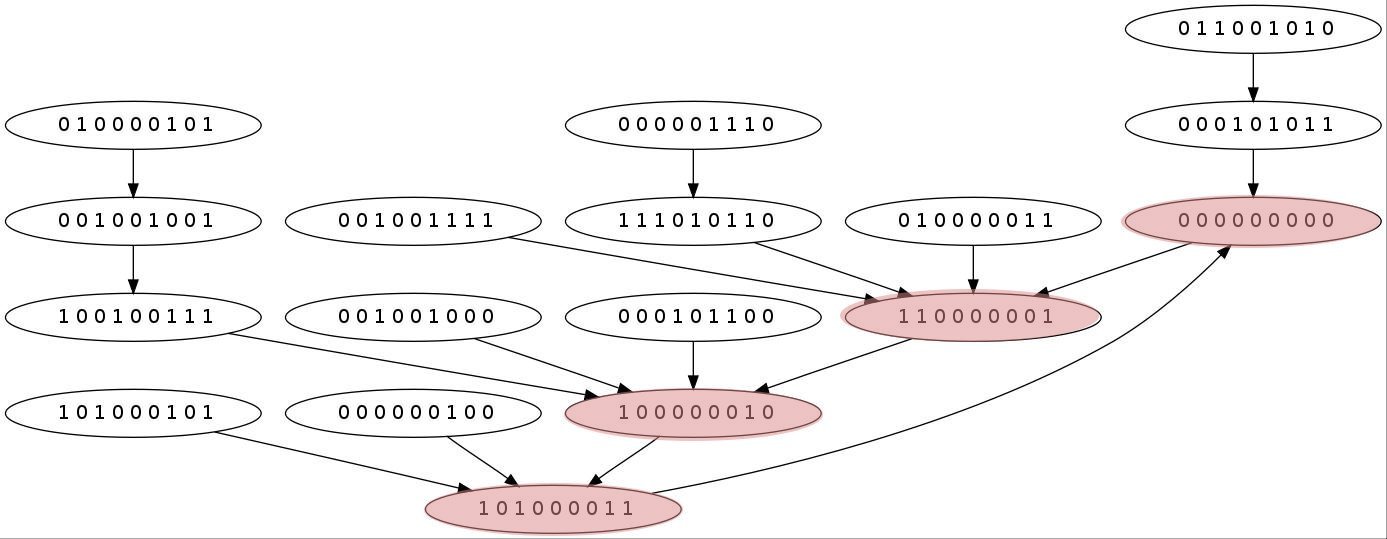
\includegraphics[width = 0.7\textwidth]{network.jpg}
\end{figure}
\end{frame}

\begin{frame}
 \frametitle{Array}
\begin{equation}
                f_1 = \left\{
                \begin{array}{l l l}
                (0,0) & \rightarrow & 0\\
                (0,1) & \rightarrow & 1\\
                (1,0) & \rightarrow & 1\\
                (1,1) & \rightarrow & 0\\
                \end{array} \right.
\end{equation}
\end{frame}

\begin{frame}
	\frametitle{Simple Example}
\begin{columns}
  \begin{column}[l]{0.5\textwidth}
	\begin{figure}
		\centering
		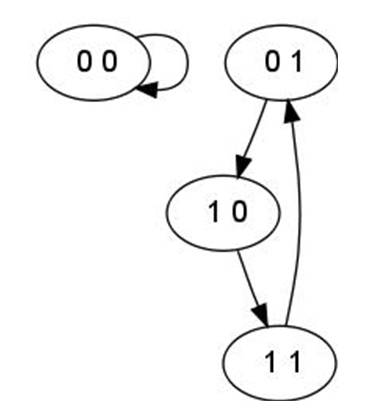
\includegraphics[height=1in,width=1in]{2by2Ex_statespace.jpg}
		\caption{State space for a 2 by 2 system}
	\end{figure}
	\end{column}
	
	\begin{column}[r]{0.5\textwidth}
	\begin{figure}
 		\centering
		\includegraphics[height=1in,width=2in]{2by2Ex_table.jpg}
		\caption{Truth table for 2 by 2 system}
	\end{figure}
	\end{column}
\end{columns}
\end{frame}

\begin{frame}
	\frametitle{Simple Example}
%	\begin{equation}
%		f_1 = \left\{ 
%		\begin{array}{l l 1}
%  		(0,0) & \rightarrow & 0\\
%  		(0,1) & \rightarrow & 1\\
%  		(1,0) & \rightarrow & 1\\
%  		(1,1) & \rightarrow & 0\\
%		\end{array} \right.
%	\end{equation}\\
	\vspace{-20pt}
	\begin{figure}
	\centering
		\includegraphics[height=1.2in,width=1.75in]{boolfunction.png}
	\end{figure}
	We can write any boolean function defined in this way as a polynomial $f:\mathbb{F}_2^2\rightarrow\mathbb{F}_2^2$ where\\
	\begin{equation*}
		 f_1(x1,x2) = \sum_{i=1}^4 b_i \prod_{j=1}^2 (1 - (c_{i,j} - x_i))
	\end{equation*}\\
	where $c_{i,j}$ are the $i,j$th entries into the matrix {\color{red}$C$} and $b_i$ are the $i$th entries into the vector {\color{blue}$B$}.\\
%		\begin{equation*}
%		C = \begin{pmatrix}
%  		0 & 0\\
%  		0 & 1\\
%  		1 & 0\\
%  		1 & 1 
% 			\end{pmatrix}
%		\end{equation*}\\
\end{frame}

\begin{frame}
	\frametitle{Simple Example}
	Then
	\begin{align*}
	f_1 &= 0*(1-(0-x_1)(1-(0-x_1)) \\
	&+ 1*(1-(0-x_1))(1-(1-x_2)) \\
	&+ 1*(1-(1-x_1))(1-(0-x_2)) \\
	&+ 0*(1-(1-x_1))(1-(1-x_2))\\ \\
	&= (1-x_1)x_2 + x_1(1-x_2)\\ \\
	&= x1+x2\\ 
	\end{align*}
	This is a polynomial in $\mathbb{F}_2^2$.
\end{frame}

\begin{frame}
	\frametitle{How to Find Fixed Points}
	Consider the single fixed point:
	\begin{figure}
		\centering
		\includegraphics[height=.6in,width=.75in]{fixedpoint.png}
	\end{figure}
	To determine a fixed point we set $f_i=x_i$ $\forall$ $i=1,\ldots,n$
\end{frame}

\begin{frame}
	\frametitle{Groebner Bases}
	Key Idea: We want to simplify the analysis of finding fixed points by computing a bases for the polynomials $f_1-x_1,\ldots,f_n-x_n$\\
	\begin{itemize}
		\item{Let $f$, $g$ be polynomials in one variable. Then we can write $f=qg+r$ where $q$ and $r$ are unique polynomials.}\\
		\item{This means there is an algorithm for finding the remainder, $r$.}\\
		\item{But in general the remainder is not unique in division with polynomials in more than one variable.}\\
	\end{itemize}
	Groebner bases allow for a unique remainder which means we can compute them by computer algebra system.\\	 
%		\item{Given functions $f_1,\ldots,f_n$ which define some biological system we can compute the
%		Groebner basis $G=<g_1,\ldots,g_t>$ by a computer algorithm system like Macaulay2.}\\
%		\item{This simplifies the analysis to $g_i=0$ $\forall$ $i=1,\ldots,t$}
\end{frame}

\begin{frame}
	\frametitle{How Groebner Bases Simplify the Analysis}
	\begin{itemize}
		\item{Groebner bases are functions in triangular form where often the first equation is only in one variable. This means you can solve the 			     system by back substitution.}\\ 
		\item{As an example consider the functions:\\ $f_1=xy+x+y+1$ and $f_2=xy+x+1$.}\\
		\item{The Groebner basis is $g_1=y$ and $g_2=x+1$ which is easily solvable by back substitution.}\\ $y=0$ and $x=1$.
	\end{itemize}
\end{frame}

\begin{frame}
	\frametitle{Recap}
	\begin{figure}
 		\centering
		\includegraphics[width=4.6in]{flowchart.jpg}
	\end{figure}
\end{frame}

\begin{frame}
 \frametitle{Goals - What We Hope to Accomplish}

	Over the next eight weeks we will\\
	\begin{itemize}
	
		\item{Develop mathematical algorithms to analyze dynamics of large biological networks}
		\item{Write a software package using Macaulay2}
		\item{Incorporate our software with exisiting programs}
			\begin{itemize}
				\item{GINsim}
				\item{Polynome}
				\item{Petrinet software}
			\end{itemize}
	\end{itemize}

\end{frame}

\begin{frame}
\frametitle{After the software is written}

	Verify the usefulness of the software\\
		\begin{itemize}
			\item{Build a boolean model given a biological system}
			\item{Use the software we will write to analyze the dynamics of the system}
				\begin{itemize}
			\item{Find the longest limit cycle}
			\item{Calculate the number of components}
			\item{Find all fixed points}
				\end{itemize}
		\end{itemize}

\end{frame}

\begin{frame}
\frametitle{Conclusion}

	\begin{itemize}
		\item{As we can express biological systems as polynomial functions we can implement abstract algebra to provide us 				with mathematical tools}
		\item{Developing the software is necessary to analyze large biological systems}	
		\item{To develop software we will need mathematical algorithms that allow one to analyze large biological systems in a 			systematic way} 
		\item{Software will be user friendly with easy to use interface}
		\item{Any biologist or other professional will be able to input the functions of a model that he or she wishes to know 			the key dynamics of}
	\end{itemize}
\end{frame}

\end{document}
